\noindent As Figure \ref{fig:introdiag} shows, some layers' activations are binarizable (produce lower error when binarized) while other layers give high binarization errors. In this chapter, we will explore the second question: Which layers are more important than other layers in a network?

\begin{figure}[h]
\centering
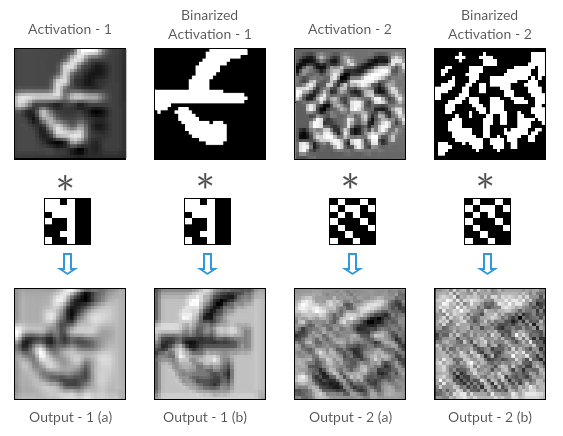
\includegraphics[width=0.8\textwidth]{figures/Intro-Diagram.png}
\caption{Convolution of binary and non-binary activations of two different layers. Note that the error introduced due to binarization is minimal in the first pair compared to the second. Hence, efficiently deciding \textit{which} layers to binarize could contribute significantly to the overall accuracy of the network and not damage the speed-ups.}
\label{fig:introdiag}
\end{figure}

\section{Hybrid Binarization}

\noindent We define certain conventions to be used throughout the paper. We define a WBin CNN to be a CNN having the weights of convolutional layers binarized (referred to as WeightBinConv layers), FBin CNN to be a CNN having both inputs and weights of convolutional layers binarized (referred to as FullBinConv layers) and FPrec CNN to be the original full-precision network having both weights and inputs of convolutional layers in full-precision (referred to as Conv layers). We compare the FBin and WBin networks with FPrec networks at specific layers.\\

\noindent Table \ref{table:versions_imagenet} and Table \ref{table:tub_recacc} in the Experiments section show test accuracies for WBin, FBin and FPrec networks of different models. Observe that there is very little loss in accuracy from FPrec to WBin networks with significant memory compression and fewer FLOPs. However, as we go from WBin to FBin networks, there is a significant drop in accuracy along with the trade-off of significantly lower FLOPs in FBin over WBin networks. Hence, we focus on improving the accuracies of FBin networks along with preserving the lower FLOPs as far as possible by investigating which activations to binarize.


\begin{figure}[t]
\centering
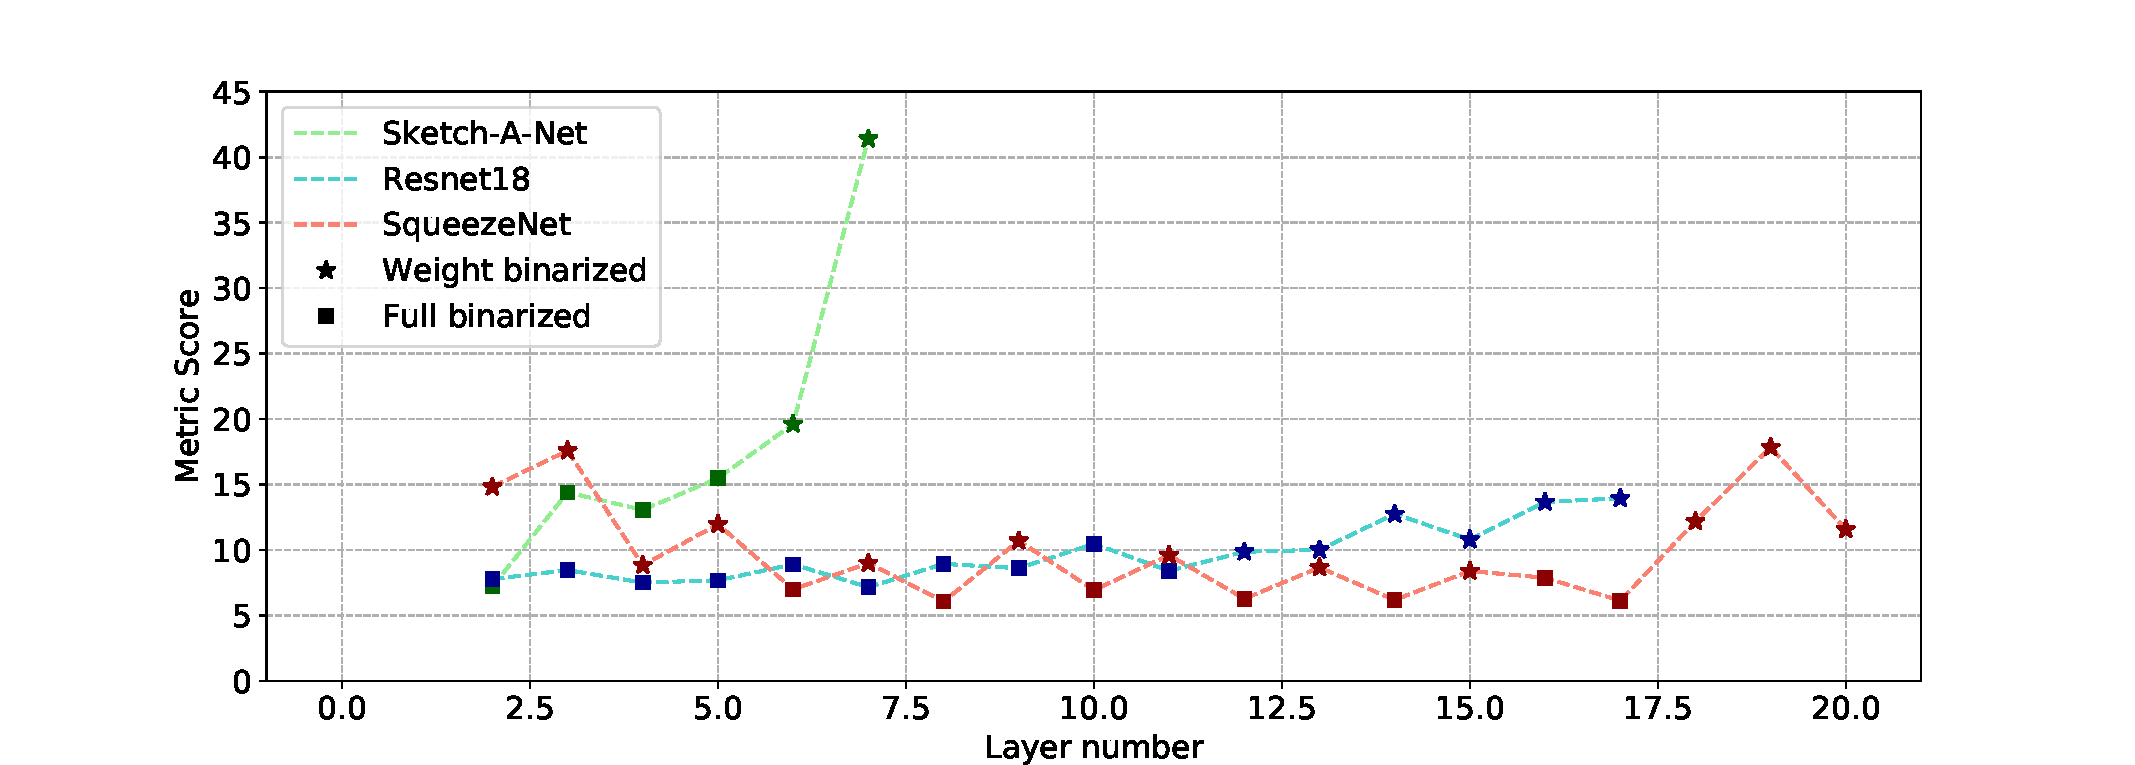
\includegraphics[width=1.0\columnwidth]{figures/metric.pdf}
\caption{Binarization-error metric across layers for Sketch-A-Net, ResNet-18, and SqueezeNet. Stars indicate that the layer was replaced with a WeightBinConv layer, while squares indicate the FullBinConv layer was retained in the FBin model. We see that the algorithm selects the last layers in the case of Sketch-A-Net and ResNet, while in the case of SqueezeNet, it selects the first four, last three and some alternate intermediate layers to be replaced by WeightBinConv layers, retaining the rest  as FullBinConv layers.}
\label{fig:metric}
\end{figure}

\subsection{Error Metric: Optimizing Speed \& Accuracy}
\noindent Full-precision inputs $\mathbf{I} \in \mathbb{R}^n$, are approximated by binary matrix $\mathbf{I_B} \in \mathbb\{-1,+1\}^n$. The optimal binary representation $\mathbf{I_B}$ is calculated by
\begin{equation}\mathbf{I_B}^\ast  = argmin(\parallel\mathbf{I}-\mathbf{I_B}\parallel^2)\end{equation}
XNOR-Net\cite{rastegari2016xnor} minimized the error function:
\begin{equation} \mathbf{E} = \frac{\parallel \mathbf{I} - \mathbf{I_B} \parallel^2}{n}\end{equation}
In order to do that, they maximized $\mathbf{I}^\top\mathbf{I_B}$ and proposed the binary activation $\mathbf{I_B}$ to be 
\begin{equation}\mathbf{I_B}^\ast = \underset{\mathbf{\mathbf{I_B}}}{\mathrm{argmax}}(\mathbf{I}^\top\mathbf{I_B}), \mathbf{I_B} \in \{-1,+1\}^n , \mathbf{I} \in \mathbb{R}^n \end{equation}, obtaining the optimal $\mathbf{I_B}^\ast$ can be shown to be  $sgn(\mathbf{I}).$\\ 

\noindent We need to investigate {\it where} to replace FullBinConv with WeightBinConv layers. In order to optimize for accuracy, we need to measure the efficacy of the binary approximation for inputs to any given layer. A good metric of this is the average error function calculated over a subset of training images $\mathbf{E}$ (defined in Eq. 2) used to calculate the optimal $I_B$ itself, which is explicitly being minimized in the process. Hence, we use that error function to capture the binarization error.\\

\noindent Similarly to optimize speed, we need to convert layers with low number of FLOPs to WeightBinConv and layers having high number of FLOPs should be kept in FullBinConv. Since we need to jointly optimize both, we propose a metric that tries to achieve a good tradeoff between the two quantities. A simple but effective metric is the linear combination \begin{equation} \mathbf{M} = \mathbf{E} + \gamma \cdot \frac{1}{\mathbf{NF}} \end{equation} where $\gamma$ is the tradeoff ratio, $\mathbf{NF}$ is the number of flops in the layer and $\mathbf{E}$ is the binarization error per neuron. The trade-off ratio $\gamma$ is a hyperparameter which ensures that both the terms are of comparable magnitude. Figure \ref{fig:metric}, captures the layer-wise variation of the error metric across multiple models.

\subsection{Partitioning Algorithm}

\noindent We aim to partition the layers of a network into two parts, one set of layers to keep FullBinConv and the other set which are replaced with WeightBinConv layers. A naive but intuitive partitioning algorithm would be to sort the list of metric errors {\bf $M$} and replace FullBinConv layers which have highest error values {\bf $M_i$} one-by-one with WeightBinConv layers, train new hybrid models and stop when the accuracies in the retrained models stop improving i.e when the maxima in accuracy v/s flops tradeoff is reached. However, we need a partitioning algorithm which gives informed guesses on where are the effective places to partition the set. This would avoid the long retraining times and large resources required to try every possible option for a hybrid model. We propose a layer selection algorithm that gives informed partitions from a trained FBin model, helping us to determine which layers are to be converted to WeightBinConv and which layers are to be converted to FullBinConv without having to train all possible hybrid models from scratch.\\

\begin{algorithm}[t]
\centering
\caption{{\bf Partition Algorithm} \\Marks layers for binarization and creates a hybrid network.}
\begin{algorithmic}[1]
\State Inputs $\Rightarrow$Layer-wise Binarization Errors
\\

\State \texttt{Initialization}
\State $P$ = Total convolutional layers
\State $R$ = Hybridization Ratio
\State ToConvert = List() \\
\State \texttt{Mark binary layers}
\For{$N$ = 2 to P}
	\State Compute KMeans with $N$ means
	\State $K$ = Number of layers in highest-error cluster
	\If{$K/P \leq R$}
	\For{$Q$ in high-error clusters}
        	\State ToConvert.add($Q$) \Comment{Add layer $Q$ }
    \EndFor
    \State Break
	\EndIf
\EndFor 

\\

\State \texttt{Create Hybrid Network}
\State HybridNet = ()

\State HybridNet.Add(Conv)
\\
\For{$N$ = 2 to P}
        \If{$N$ in ToConvert}
            \State HybridNet.Add(WeightBinConv)
        \Else
        	\State HybridNet.Add(FullBinConv)
        \EndIf
\EndFor
\\
\State Output $\Rightarrow$ HybridNet

\end{algorithmic}
\label{alg:partitionalgo}
%\vspace*{-0.75cm}
\end{algorithm}
\begin{figure}[t]
\centering
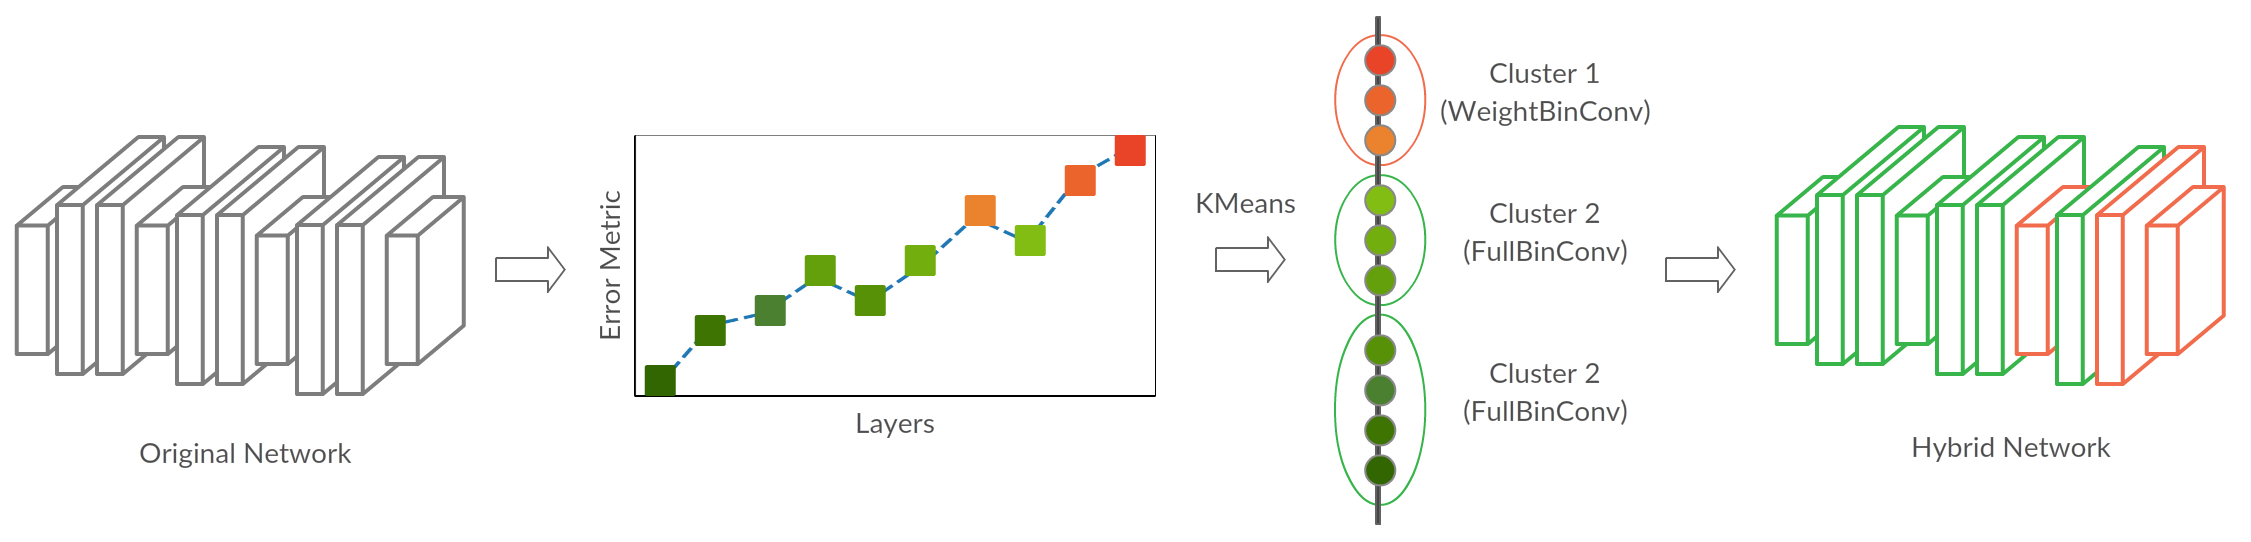
\includegraphics[width=1.0\textwidth]{figures/Main-Algo-Diagram.png}
\caption{The Procedure: Error metrics from binarization of inputs to the network layers are partitioned into clusters using K-means. The highest error cluster indicates the inputs that are not binarized to generate the hybrid version.}
\label{fig:pipeline}
%\vspace{-1.5cm}
\end{figure}
\noindent Our algorithm starts by taking a trained FBin model. We pass in a subset of the training images and calculate the average error metric for all layers over them. Then we perform K-Means Clustering on the metric values with each point being the metric error of layers as shown in Figure \ref{fig:metric}. We perform the K-Means Clustering for different values of the number of clusters. We find a suitable number of clusters such that the ratio of layers in the highest-error cluster ($K$) to the total number of convolutional layers ($P$) is less than a hyperparameter, which we define as the Hybridization Ratio $R$. Layers with terms falling in the highest mean cluster are converted to WeightBinConv, while the ones in all other clusters are left as FullBinConv. A flow of the algorithm is illustrated in Figure \ref{fig:pipeline} and is explained step-by-step in Algorithm \ref{alg:partitionalgo}. We show metric scores of various layers for different networks in Figure \ref{fig:metric} and indicate which layers are replaced with WeightBinConv/FullBinConv layers. This algorithm guides in forming the architecture of the hybrid model, which is then trained from scratch obtaining the accuracies given in the tables presented in the Experiment section. Note that this algorithm does not change the configuration of the model; it only converts certain layers to their binarized versions.\\

\noindent To give an intuition of what the Hybridization ratio $R$ means, a low $R$ would indicate we need the number of WeightBinConv layers to be low, ensuring a high asymmetry between errors in WeightBinConv and FullBinConv layers, prioritizing saving computational cost. Conversely, a higher $R$ would prioritize accuracy over computational cost. $R$ was set to be 0.4 for AlexNet and ResNet-18, and 0.6 for Squeezenet. Variation with different values of $R$ is further discussed in the experiments section.

\subsection{Impact on Speed and Energy Use}
\noindent {\bf Computational Speedups}: Convolutional operations are computationally expensive. For each convolution operation between an image $\mathbf{I} \in \mathbb{R}^{c_{in} \times h_I \times w_I}$ and weight $\mathbf{W} \in \mathbb{R}^{c_{out} \times h \times w}$, the number of MAC operations required $N$ are $\approx C_{in}C_{out}N_WN_I$ where $N_W = wh$ and $N_I = w_Ih_I$. According to benchmarks done in XNOR-Net, the current speedup obtained in these operations is 58x after including the overhead induced by computing $\alpha$. Accordingly, in later sections, we take one FLOP through a layer as equivalent to 58 binary operations when weights and inputs are binarized. \\ 

\noindent {\bf Exploiting filter repetitions}: The number of unique convolutional binary filters is bounded by the size of the filter \cite{courbariaux2016binarized}. As most of our intermediate convolutional layers have $3\times3$ filters which only have $2^9$ unique filters, we find that the percentage of unique filters decreases as we go deeper into the network. We can exploit this fact to simply prune filters and use that in calculating speedups for binary networks. More details regarding how the speedup was computed is included in the supplementary material.

%------------------------------------------------------------------------
\section{Experiments and Results}

\noindent We report and compare accuracies, speedups and compression between the FPrec model, different kinds of binarization models (WBin and FBin), and their generated hybrid versions of the same. We also present a detailed comparison of our method with several different compression techniques applied on AlexNet \cite{alex2012alexnet}, ResNet-18 \cite{he2016deep}, Sketch-A-Net \cite{eitz2012hdhso} and SqueezeNet \cite{iandola2016squeezenet}. \\

\noindent We empirically demonstrate the effectiveness of hybrid binarization on several benchmark image and sketch datasets. We show that our approach is robust and can generalize to different types of CNN architectures across domains.

\subsection{Datasets and Models}
\noindent Binary Networks have achieved accuracies comparable to full-precision networks on limited domain/simplified datasets like CIFAR-10, MNIST, SVHN, but show drastic accuracy losses on larger-scale datasets. To compare with state-of-the-art vision, we evaluate our method on ImageNet\cite{deng2009imagenet}. To show the robustness of our approach, we test it on sketch datasets, where models fine-tuned with ImageNet are demonstrably not suitable as shown in\cite{yu2015sketch}. Binary networks might be better suited for sketch data due to its binary nature and sparsity of information in the data. \\

\noindent {\bf ImageNet:} The benchmark dataset for evaluating image recognition tasks, with over a million training images and 50,000 validation images. We report the single-center-crop validation errors of the final models.\\

\noindent {\bf TU-Berlin:} The TU-Berlin \cite{eitz2012hdhso} sketch dataset is the most popular large-scale free-hand sketch dataset containing sketches of 250 categories, with a human sketch-recognition accuracy of 73.1\% on average.\\ 

\noindent {\bf Sketchy:} It is a recent large-scale free-hand sketch dataset containing 75,471 hand-drawn sketches from across 125 categories. This dataset was primarily used to cross-validate results obtained on the TU-Berlin dataset and ensure that our approach is robust to the variation in collection of data.\\

\begin{table}[t]
\centering
\begin{tabular}{|l|c|c|c|c|l|}
\hline
{\bf Technique} & {\bf Acc-Top1} & {\bf Acc-Top5} & {\bf W/I} & {\bf Mem} & {\bf FLOPs} \\
\hline
\multicolumn{6}{|c|}{\sc { \bf AlexNet}} \\
\hline
BNN & 39.5\% & 63.6\% & 1/1 & 32x & 121 (1x)\\
XNOR & 43.3\% & 68.4\% & 1/1 & 10.4x & {\bf 121 (1x)} \\
Hybrid-1 & 48.6\% & 72.1\% & 1/1 & 10.4x & 174 (1.4x)\\
Hybrid-2 & {\bf 48.2\%} & {\bf 71.9\%} & 1/1 & {\bf 31.6x} & 174 (1.4x)\\
\hline
HTCBN & 46.6\% & 71.1\% & 1/2 & 31.6x & 780 (6.4x)\\
DoReFa-Net & 47.7\% & - & 1/2 & 10.4x & 780 (6.4x)\\
\hline
\multicolumn{6}{|c|}{\sc { \bf Res-Net 18}} \\
\hline
BNN & 42.1\% & 67.1\% & 1/1 & 32x & 134 (1x)\\
XNOR & 51.2\% & 73.2\% & 1/1 & 13.4x & {\bf 134 (1x)} \\
Hybrid-1 & 54.9\% & 77.9\% & 1/1 & 13.4x & 359 (2.7x)\\
Hybrid-2 & {\bf 54.8\%} & {\bf 77.7\%} & 1/1 & {\bf 31.2x} & 359 (2.7x)\\
\hline
HTCBN & 53.6\% & - & 1/2 & 31.2x & 1030 (7.7x)\\
\hline
\end{tabular}
\caption{
A detailed comparison of accuracy, memory use, FLOPs with popular benchmark compression techniques on ImageNet. Our hybrid models outperform other 1-bit activation models and perform on par with 2-bit models while having a significantly higher speedup. Hybrid-2 models have the last layer binarized.}
\label{table:imagenet_fullcomp}
\end{table}

\noindent We use the standard splits with commonly used hyper-parameters to train our models. Each FullBinConv block was structured as in XNOR-Net (Batchnorm-Activ-Conv-ReLU). Each WeightBinConv and Conv block has the standard convolutional block structure (Conv-Batchnorm-ReLU). Weights of all layers except the first were binarized throughout our experiments unless specified otherwise. Note that FLOPs are stated in millions in all diagrams and sections. All networks are trained from scratch independently. The architecture of the hybrid network once designed does not change during training. Additional details about the datasets, model selection and layer-wise description of each of the hybrid models along with experimental details can be found in the supplementary material. 

\subsection{Results}

\noindent We compare FBin, WBin, Hybrid and FPrec recognition accuracies across models on ImageNet, TU-Berlin and Sketchy datasets. Note that higher accuracies are an improvement, hence stated in green in the table, while higher FLOPs mean more computational expense, hence are stated in red. W/I indicates the number of bits used for weights and inputs to the layer respectively. Note that in the table, the compression obtained is only due to the weight binarization, while the decrease in effective FLOPs are due to activation binarization.\\

\noindent On the ImageNet dataset in Table \ref{table:versions_imagenet}, hybrid versions of AlexNet and ResNet-18 models outperform their FBin counterparts in top-1 accuracy by 4.1\% and 3.6\% respectively, and around 20x compression for both. We also compare with the results of other compression techniques in Table \ref{table:imagenet_fullcomp}.\\

\begin{table}[t]
\centering
\begin{tabular}{|l|c|c|c|c|l|}
\hline
\multirow{2}{*}{\bf Model} & \multirow{2}{*}{\bf Method} & \multicolumn{2}{c|}{\sc { \bf Accuracy}} & \multirow{2}{*}{\bf Mem} & \multirow{2}{*}{\bf FLOPs}\\
\cline{3-4}
 &  & Top-1 & Top-5 &   &  \\
\hline
\multirow{5}{*}{AlexNet} & FPrec & 57.1\% & 80.2\% & 1x & 1135 (9.4x)\\
 & WBin (BWN) & 56.8\% & 79.4\% & 10.4x & 780 (6.4x)\\
 & FBin (XNOR) & 43.3\% & 68.4\% & 10.4x & {\bf 121 (1x)} \\
 & Hybrid-1 &  48.6\% & 72.1\% & 10.4x & 174 (1.4x)\\
 & Hybrid-2 & {\bf  48.2\%} & {\bf 71.9\%} & {\bf 31.6x} & 174 (1.4x)\\
\hline
Increase & Hybrid vs FBin & +4.9\% & +3.5\% & +21.2x & +53 (+0.4x) \\
\hline
\multirow{5}{*}{ResNet-18} & FPrec & 69.3\% & 89.2\% & 1x & 1814 (13.5x)\\
 & WBin (BWN) & 60.8\% & 83.0\% & 13.4x & 1030 (7.7x)\\
 & FBin (XNOR) & 51.2\% & 73.2\% & 13.4x & {\bf 134 (1x)}\\
 & Hybrid-1 & 54.9\% & 77.9\% & 13.4x & 359 (2.7x)\\
 & Hybrid-2 & {\bf 54.8\%} & {\bf 77.7\%} & {\bf 31.2x} & 359 (2.7x)\\
\hline
Increase & Hybrid vs FBin & +3.6\% & +4.5\% & +17.8x & +225 (+1.7x)\\
\hline
\end{tabular}
\caption{Our hybrid models compared to FBin, WBin and NoBin models on Imagenet in terms of accuracy, memory and computations expense.}
\label{table:versions_imagenet}
\end{table}

\begin{table}[t]
\centering
\begin{tabular}{|l|c|c|c|c|l|}
\hline
\multirow{2}{*}{\bf Model} & \multirow{2}{*}{\bf Method} & \multicolumn{2}{c|}{\sc { \bf Accuracy}} & \multirow{2}{*}{\bf Mem} & \multirow{2}{*}{\bf FLOPs}\\
\cline{3-4}
 &  & TU-Berlin & Sketchy &  &  \\
\hline
\multirow{4}{*}{Sketch-A-Net} & FPrec & 72.9\% & 85.9\% & 1x & 608 (7.8x)\\
 & WBin (BWN) & 73\% & 85.6\% & 29.2x & 406 (5.2x)\\
% & FBin (XNOR) & 48.2\% & 38.6\% & 29.2x & 78 (1x) \\
 & FBin (XNOR) & 59.6\% & 68.6\% & 19.7x & {\bf 78 (1x)} \\
 & Hybrid & {\bf 73.1\%} & {\bf 83.6\%} & {\bf 29.2x} & {\bf 85 (1.1x)}\\
\hline
Increase & Hybrid vs FBin & +13.5\% & +15.0\% & +9.5x & +7 (+0.1x)\\
\hline
\multirow{4}{*}{ResNet-18} & FPrec & 74.1\% & 88.7\% & 1x & 1814 (13.5x) \\
 & WBin (BWN) & 73.4\% & 89.3\% & 31.2x & 1030 (7.7x)\\
 & FBin (XNOR) & 68.8\% & 82.8\% & 31.2x & {\bf 134 (1x)} \\
 & Hybrid  & {\bf 73.8\%} & {\bf 87.9\%} & {\bf 31.2x} & 359 (2.7x)\\
\hline
Increase & Hybrid vs FBin & +5.0\% & +5.1\% & - & +225 (+1.7x)\\
\hline
\end{tabular}
\caption{Our hybrid models compared to FBin, WBin and full prec models on TU-Berlin and Sketchy datasets in terms of accuracy, memory and speed tradeoff.} 
\label{table:tub_recacc}
\end{table}

\noindent On the TU-Berlin and Sketchy datasets in Table \ref{table:tub_recacc}, we find that Sketch-A-Net and ResNet-18 have significantly higher accuracies in the hybrid models compared to their FBin counterparts, a 13.5\% gain for Sketch-A-Net and 5.0\% for ResNet-18. \\

\noindent These hybrid models also achieve over 29x compression over FPrec models and with a reasonable increase in the number of FLOPs - a mere 7M increase in Sketch-A-Net and a decent 225M increase in ResNet-18. We also compare them with state-of-the-art sketch classification models in Table \ref{table:sketchcomp}. Our hybrid Sketch-A-Net and ResNet-18 models achieve similar accuracies to state-of-the-art, while also highly compressing the models upto 233x compared to the AlexNet FPrec model. \\

\begin{figure*}
\centering
\begin{tabular}{cc}
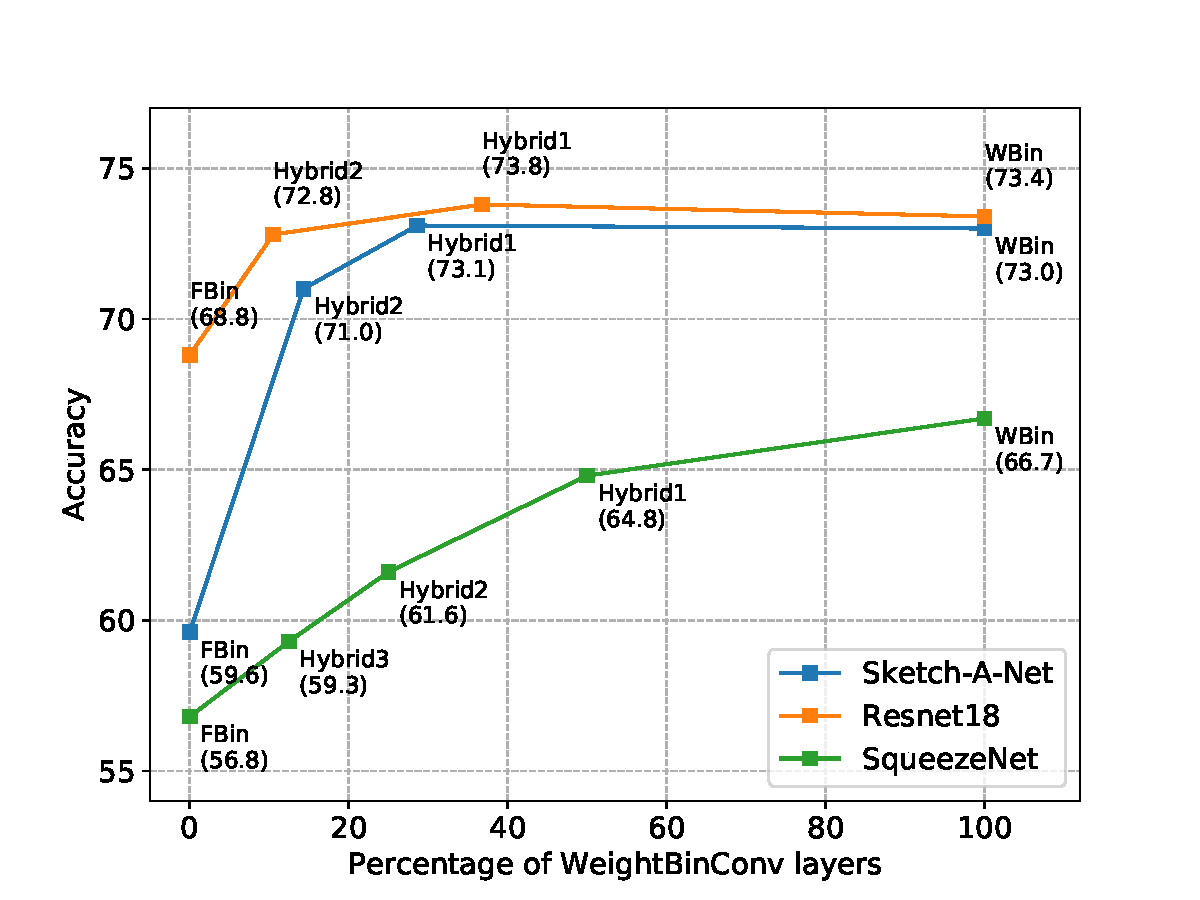
\includegraphics[width=0.5\textwidth]{figures/Figure_1.pdf} &
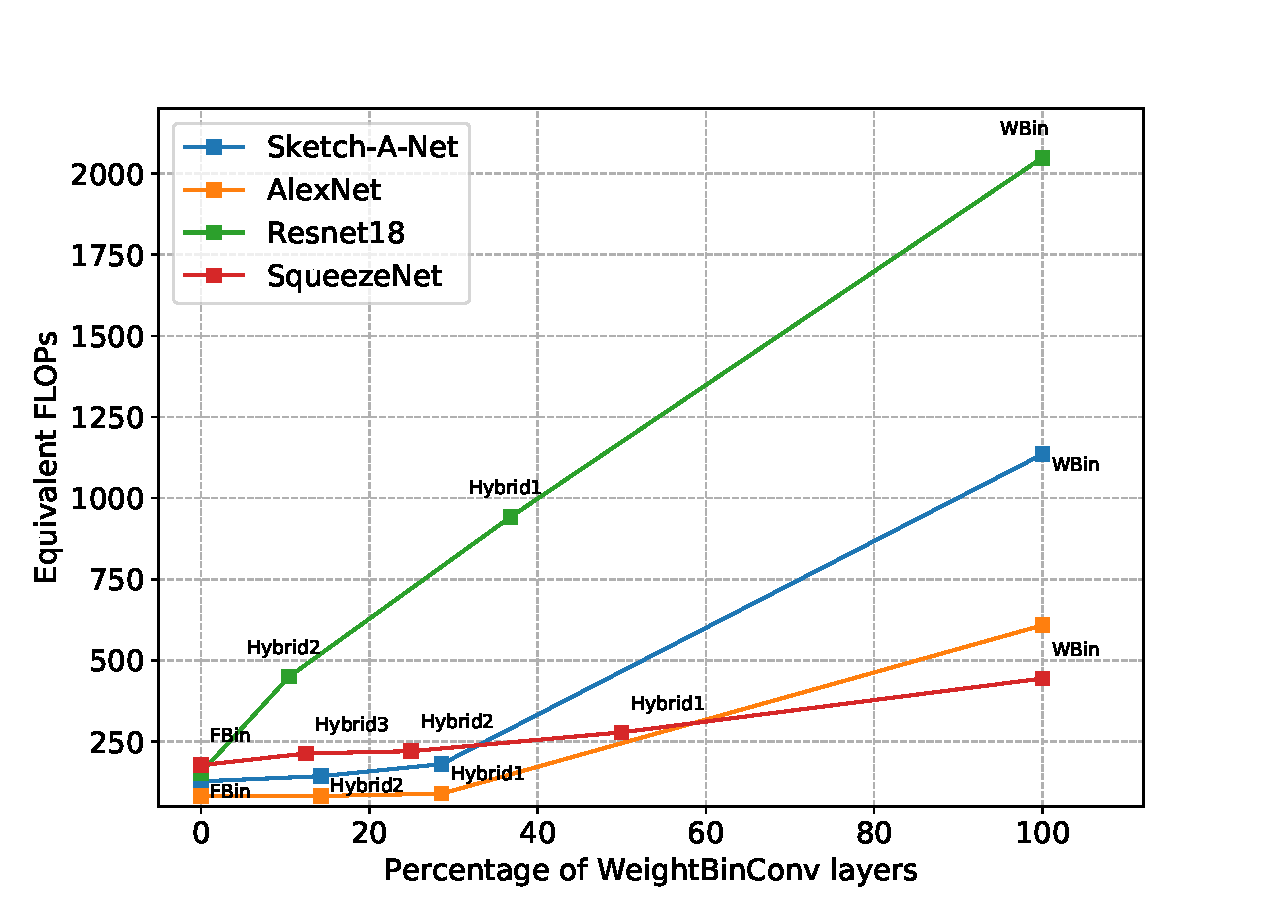
\includegraphics[width=0.5\textwidth]{figures/Figure_2.pdf}\\
\end{tabular}
\caption{Trade-off between WeightBinConv layers and accuracy on the TU-Berlin dataset is shown in the left figure, while the trade-off between weight binarized layers and speedup is shown in the right figure. Early on, we observe that a small increase in the percentage of WeightBinConv layers leads to a large increase in accuracy and a marginal decrease in speed. We achieve accuracies comparable to the WBin model with much fewer WeightBinConv layers.
}
\label{fig:tradeoff}
\end{figure*}

Thus, we find that our hybrid binarization technique finds a balance between sacrificing accuracy and gaining speedups and compression for various models on various datasets.
\begin{table}[t]
\begin{center}
\begin{tabular}{|l|c|c|c|l|}
\hline
{\bf Model} & {\bf Acc} & {\bf Mem} & {\bf FLOPs}\\
\hline
AlexNet-SVM & 67.1\% & 1x & 1135 (13.4x)\\
AlexNet-Sketch & 68.6\% & 1x & 1135 (13.4x)\\
Sketch-A-Net SC & 72.2\% & 8x & 608 (7.2x)\\
\hline
Sketch-A-Net-Hybrid & {\bf 73.1\%} & {\bf 233x} & {\bf 85 (1x)}\\
ResNet18-Hybrid & {\bf 73.8\%} & - & {\bf 359 }\\
\hline
Humans & {73.1\%} & - & - \\
Sketch-A-Net-2  \footnotemark \cite{yu2017sketch} & {\bf 77.0\%} & 8x & 608 (7.2x)\\
\hline
\end{tabular}
\footnotetext{It is the sketch-a-net SC model trained with additional imagenet data, additional data augmentation strategies and considering an ensemble, hence would not be a direct comparison}
\end{center}
\caption{A comparison between state-of-the-art single model accuracies of recognition systems on the TU-Berlin dataset.}
\label{table:sketchcomp}
\end{table}

\subsection{Algorithmic Insights}
\noindent We gained some insights into where to binarize from our investigation. We provide them as a set of practical guidelines to enable rapid prototyping of hybrid models, which gives meaningful insights into which layers were partitioned.\\

\noindent {\bf Convert layers towards the end to WeightBinConv:} It is observed that later layers typically have high error rates, more filter repetitions, and lower computational cost. Hence, the algorithm tends to start converting models to Hybrid from the last layers. \\

\noindent {\bf Convert the smaller of the layer placed parallely to WeightBinConv:} It is a good idea to convert the smaller of the parallely placed layers in the architecture like Residual layers in the ResNet architecture to WeightBinConv, since converting them to WeightBinConv would not damage the computational speedup obtained by the parallel FullBinConv layers.\\

\noindent {\bf Pick a low Hybridization Ratio:} Try to pick low values of the Hybridization Ratio $R$, ensuring a low proportion of number of layers the highest-error cluster.\\

\noindent {\bf Relax the Hybridization Ratio for compact models:} Having a higher Hybridization Ratio for compact models which inherently have fewer flops leaves more layer inputs un-binarized and retains accuracy. 

\subsection{Why are layer-wise errors independent?}
\noindent Can binarization noise introduced in a layer propagate further into the network and influence other layers? Courbariaux \etal \cite{courbariaux2016binarized} provide some insights for the same. Let $\mathbf{W}$ be the weight and $\mathbf{I}$ be the input to the convolutional layer. The output of the convolution between the binary weights and inputs can be represented by \begin{equation}\mathbf{O_B} = \alpha \cdot (sgn(\mathbf{W}^\intercal) \odot sgn(\mathbf{I}))\end{equation} The desired output $\mathbf{O}$ is modelled by $\mathbf{O_B}$ along with the binarization noise $\mathbf{N}$ introduced due to the function $sgn(.)$. \begin{equation}\mathbf{O} = \mathbf{W} * \mathbf{I} = \sum_{i}^{} \mathbf{O_B}_i + \mathbf{N_i}\end{equation} When the layer is wide, we expect the deterministic term $\mathbf{O_B}$ to dominate, because the noise term $\mathbf{N}$ is a summation over many independent binarizations from all the neurons in the layer. Thus, we argue that the binarization noise $\mathbf{N}$ should have minimal propagation and do little to influence the further inputs. Hence, it is a reasonable approximation to consider the error across each layer independently of the other layers.

\subsection{Variation with the Hybridization Ratio ($R$)}
\noindent To observe the trade-off between accuracy and speedup on different degrees of binarization, we chose different values of the Hybridization Ratio ($R$) to create multiple hybrid versions of the AlexNet, ResNet-18 and SqueezeNet models. Picking a larger $R$ would result in a higher number of WeightBinConv layers. We compare these hybrid networks to their corresponding FBin and WBin versions. \\

\noindent In Figure \ref{fig:tradeoff}, we show model accuracies of AlexNet, ResNet-18 and SqueezeNet on the ImageNet dataset plotted against the number of WeightBinConv layers, starting from only FBin versions on the left, to only WBin versions on the right. We observe that in the case of AlexNet and ResNet-18, which are large models, we recover WBin accuracies quickly, at around the 35\% mark (Roughly a third of the network containing WeightBinConv layers), with low computational trade-off. We also observe that on sketch data, hybrid models tend to perform significantly better and perform on par with their WBin counterparts.\\ 

\noindent We also notice that the smaller a model, the more trade-off must be made to achieve WBin accuracy, i.e a larger Hybridization Ratio must be used. AlexNet, the largest model crosses WBin accuracy at around 32\%, while ResNet-18, being smaller, saturates at around 40\%. SqueezeNet, a much more compact model, reaches its WBin accuracy at 60\%.

\subsection{Optimizing Memory}
\noindent We measured accuracies for FBin and Hybrid variants of Sketch-A-Net and ResNet-18 models on TU-Berlin and Sketchy Datasets with weights of the last layer binarized as well as non-binarized and the results are presented in Table \ref{table:otherresults}. For AlexNet-styled architectures (Sketch-A-Net), we observe a drastic drop in accuracies (From 59.1\% to 48.3\%) on binarizing the last layer, similar to observations made in previous binarization works \cite{zhou2016dorefa,tang2017train}. \\

\begin{table}[t]
  \centering
\begin{tabular}{|l|c|c|c|c|c|}

\hline
{\bf Model} & {\bf BinType} & {\bf Last Bin?} & {\bf Acc } & {\bf Mem}\\
\hline
\multirow{2}{*}{Sketch-A-Net} & \multirow{2}{*}{FBin (XNOR)} & No & 59.6\% & 19.7x \\
 &  & Yes & 48.3\% & {\bf 29.2x} \\

\hline
\multirow{2}{*}{Sketch-A-Net} & \multirow{2}{*}{Hybrid} & No & 73.1\% & 19.7x \\
 &  & Yes & 72.0\% & {\bf 29.2x} \\
\hline
\multirow{2}{*}{Resnet-18} & \multirow{2}{*}{FBin (XNOR)} & No & 69.9\% & 13.4x \\
 &  & Yes & 68.8\% & {\bf 31.2x} \\

\hline
\multirow{2}{*}{Resnet-18} & \multirow{2}{*}{Hybrid} & No & 73.9\% & 13.4x \\
 &  & Yes & 73.8\% & {\bf 31.2x} \\
\hline
\end{tabular}
\caption{Effects of last layer weight-binarization on TU-Berlin dataset, for Sketch-A-Net and ResNet-1. Observe that our hybrid models do not face drastic accuracy drop when the last layer is weight-binarized.}
\label{table:otherresults}
\end{table}

\noindent Many efforts were made to quantize the last layer and avoid this drop. DoReFaNet and XNOR-Net did not binarize the last layer choosing to incur a degradation in model compression instead while \cite{tang2017train} proposed an additional scale layer to mitigate this effect. However, our hybrid versions are able to achieve similar accuracies (a 1\% drop for hybrid Sketch-A-Net and no drop for ResNet-18 or AlexNet) since the last layer is weight binarized instead. Hence, our method preserves the overall speedup even though we only weight-binarize the last layer, owing to the comparatively smaller number of computations that occur in this layer.\\

\noindent Note that the first layer is always a full-precision Conv layer. The reasons behind this are the insights obtained from \cite{anderson2017high}. They state that the first layer of the network functions are fundamentally different than the computations being done in the rest of the network because the high variance principal components are not randomly oriented relative to the binarization. Also, since it contains fewer parameters and low computational cost, it does not affect our experiments.

\subsection{Compressing Compact Models}
\noindent Whether compact models can be compressed further, or {\it need} all of the representational power afforded through dense floating-point values is an open question asked originally by \cite{iandola2016squeezenet}. \\

\noindent We show that our hybrid-binarization technique can work in tandem with other compression techniques, which do not involve quantization of weights/activations and that hybrid binarization is possible even on compact models. We apply hybrid binarization to SqueezeNet\cite{iandola2016squeezenet} a recent model that employed various architectural design strategies to achieve compactness. SqueezeNet achieves an 8x compression on the compact architecture of Sketch-A-Net. On applying hybrid binarization we achieve a further 32x compression, an overall 256x compression with merely 6\% decrease in accuracy. This is due to the high rate of compression inherent and further compression is difficult due to the small number of parameters. After showing that efficacy of hybrid binarization in the previous section, we show that hybrid binarization can work in combination with other compression techniques here.\\

\begin{table}[t]
\centering

\begin{tabular}{|l|c|c|c|c|l|}
 \hline
\multirow{2}{*}{\bf Model} & \multirow{2}{*}{\bf Method} & \multicolumn{2}{c|}{\sc { \bf Accuracy}} & \multirow{2}{*}{\bf Mem} & \multirow{2}{*}{\bf FLOPs}\\
\cline{3-4}
 &   & TU-Berlin & Sketchy &   &  \\
\hline
Sketch-A-Net & FPrec & 72.9\% & 85.9\% & 1x & 1135 (12.3x)\\
Squeezenet & FPrec & 71.2\% & 86.5\% & 8x & 610 (6.6x)\\
Squeezenet & WBin & 66.7\% & 81.1\% & 23.7x & 412 (4.5x)\\
\hline
Squeezenet & FBin & 56.8\% & 66.0\% & 23.7x & {\bf 92 (1x)} \\
Squeezenet & Hybrid & {\bf 64.8\%} & {\bf 79.6\%} & {\bf 23.7x} & 164 (1.8x)\\
\hline
Improvement & Hybrid vs FBin & +8.0\% & +13.6\% & - & +72 (+0.8x)\\
\hline
\end{tabular}
\caption{Our performance on SqueezeNet, an explicitly compressed model architecture. Although SqueezeNet is an inherently compressed model, our method still achieves further compression on it.}
\label{table:squeezenet}
\end{table}

\noindent Results for SqueezeNet are shown in Table \ref{table:squeezenet} for the TU-Berlin and Sketchy datasets, and we see that accuracy is only slightly lower compared to the hybridized versions of ResNet-18 and Sketch-A-Net on the same. Hybrid SqueezeNet achieves a total compression of 256x. Similarly, this technique can be combined with many techniques such as HWGQ-Net \cite{cai2017deep} which proposes an alternative layer to ReLU and repeated binarization as illustrated in \cite{tang2017train} among others. Since our primary goal is to investigate the viability of hybrid binarization, these investigations- albeit interesting, are out of the scope of our current work.

%------------------------------------------------------------------------
\section{Summary}
\noindent We proposed a novel algorithm for selective binarization of CNNs, which strikes a balance between performance, memory-savings and accuracy. The accuracies of our hybrid models were on par with their corresponding full-precision networks on TU-Berlin and Sketchy datasets, while providing the benefits of network binarization in terms of speedups, compression and energy efficiency. We successfully weight-binarized the last layers without significant accuracy drops, a problem faced by previous works in this area. We also showed that we can successfully combine the advantages of our approach with other architectural compression strategies, to obtain highly efficient models with negligible accuracy penalties. 